

\documentclass[onecolumn]{article}
\usepackage{universityphysicslab2019}
\newcommand{\fn}{\ensuremath{\overrightarrow{\textbf{F}}\hspace{-2 pt}_{N} \hspace{2 pt}}}

\begin{document}

\labheading{2}{Becoming Familiar with an Oscilloscope}

\comments{An important diagnostic tools in the lab is the oscilloscope (also called an o-scope or scope for short). With an oscilloscope you can ``see" electrical signals by the visualization of the voltage signal as a function of time it creates.}

\materials{Oscilloscope, cables, signal generator(s), battery}

\noindent Oscilloscopes originally used cathode ray tubes as their display, but there has been a shift to using digital displays. (CRT tubes used to be on TV's, basically a beam of electrons is swept across a screen that glows when the beam strikes it. In the scope, the height of the beam is varied by the potential difference that is being read.) Digital scopes allow for additional features and more complicated analysis of a signal. CRT scopes are still widely used for many applications.  The essential functions of an oscilloscope are present both on a digital and CRT types. 

A signal generator creates various repeated signals which vary in strength (voltage) with time. 



\begin{enumerate}

\item Describe what the volts/division control is used for. In particular what is a division? (As a means of calibration, as we will learn many types batteries (AA, AAA, C, D etc) are a steady voltage source of about 1.6 V

\jump{1}

\item  What does the ``calibrate" knob do on the end of these controls? Why is it important to know how these are turned ``off"? 

\jump{1}

\pagebreak 

Set (and connect) the signal generator to output a sine wave with a frequency of 100 Hz.

\item What is the sec/division control used for? What range does it have? (As a means of understanding note that your signal generator would have a period of 0.01 s when $f=100$ Hz)

\jump{2}

\item When set to 0.5 ms/div, \textbf{predict} with a calculation the frequency such that complete single wave would appear across the screen:

\jump{2}

\item Now set the signal generator to this value, were you correct? Draw a sketch:

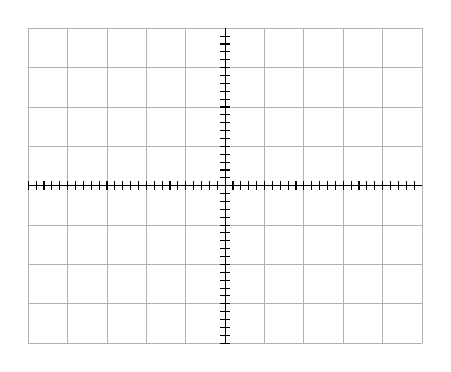
\begin{tikzpicture}
\draw[step=0.5 cm, line width=0.1mm, black!30!white] (0,0) grid (5,4);
\foreach \x in {0,0.1,...,5}{\draw (\x, 1.94) -- (\x, 2.06);}
\foreach \y in {0,0.1,...,4}{\draw (2.44,\y) -- (2.56,\y);}
\draw(0,2)--(5,2);
\draw(2.5,0)--(2.5,4);
\end{tikzpicture}

\item What is the voltage of the amplitude of this wave? Briefly explain how you can determine this: 

\jump{1}

\item What other shapes can be created on this signal generator? Sketch (generally) their output below: 
\jump{1}


\pagebreak 

\item In the next few questions we will be looking at triggering. To investigate this feature, you may want to also adjust the signal from the function generator (such as changing its strength.) Set the mode to manual also labeled normal in some models. 

\begin{enumerate}
\item What is the purpose of triggering? What does a signal look like when it is properly triggered, what about when it isn't?

\jump{1}

\item What does the triggering level knob do?

\jump{1}

\item What does the slope button in the triggering do?
\end{enumerate}

\jump{1}

\item What limit exists for the oscilloscope frequency? Describe what happens when you approach these limits. (Also note the use of the x10 feature.)

\jump{1}

%\item What is the output of the square wave on the signal generator? Set the frequency generator to square waves and examine them closely. Sketch what these waves look like.
\pagebreak 

Dual Trace: Connect two signals, one to each channel. 

\item Describe what the ``Add", ``Alt" and chop settings do. Which setting would be useful for viewing 2 signals at low frequencies? Which is better at high frequencies?

\jump{1}


\item We can plot one signal along the x-axis and the other signal along the y-axis, by selecting the X-Y feature on the timing. The result is a Lissajous figure. Lissajous figures tells us about the phase difference between the two signals and the ratio of their frequencies. You may find it difficult to maintain the Lissajous figures in a fixed configuration because the two oscillators are not phase and frequency locked. Their frequencies and phase drift slowly causing the two different signals to change slightly with respect to each other. Sketch the output of the following in X-Y mode:

\begin{enumerate}
\item {2 signals with the same frequency, in phase}
\item {2 signals with the same frequency, 180$^\circ$ out of phase}
\item {2 signals with the same frequency, 90$^\circ$ out of phase}
\item {2 sine wave signals, in phase, with one signal at 2x the frequency (a 2:1 ratio)}
\end{enumerate}

\jump{1}


\end{enumerate}
\end{document}




\subsection*{II. Oscilliscope Overview}

\subsubsection*{Background}
The strength of the electrical signal (such as sound to a speaker) can be measured by its \textbf{voltage}. Electrical signals can be observed using an oscilloscope. In the normal operation of an oscilloscope, the height of the beam is varied by the voltage, while it sweeps across the screen in a set amount of time. (Creating something like a voltage versus time graph.)To see and measure a signal on an oscilloscope, there are some key adjustments we should familiarize ourselves with: 

%\begin{center}
%\begin{tikzpicture}
%\node (img) {\includegraphics[width=12cm]{oscope}};
%\node at (-2.5,2) [rectangle,draw,fill=black!20] {A};
%\node at (0.4,2) [rectangle,draw,fill=black!20] {A};
%\node at (-2.5,-0.2) [rectangle,draw,fill=black!20] {B};
%\node at (0.4,-0.2) [rectangle,draw,fill=black!20] {B};
%\node at (2.5,-0.2) [rectangle,draw,fill=black!20] {C};
%\node at (4.2,-1.1) [rectangle,draw,fill=black!20] {D};
%\node at (-2.4,0.75) [rectangle,draw,fill=black!20] {E};
%\end{tikzpicture}
%\end{center}

\begin{enumerate}
\item[\textbf{A/B}] Vertical Amplification and Position -- The volts/div control: This knob controls the ``zoom" on the vertical axis. If you have a square wave that has an amplitude of 5 V, then a setting of 5 volts per division (5 volts/div) will show the signal go up and down by one ``box" (called a division.) If you set the volts/division control to 1 volts/div this same signal would go up and down by 5 boxes. \\

Our oscilloscopes are called dual trace oscilloscopes because they can display two different signals at the same time.  They have two separate vertical amplifiers (with independent inputs and sensitivity controls) and produce two distinct dots on the screen.  The independent inputs are designated Channel 1 (``Ch1" or ``Y in") and Channel 2 (``Ch2" or ``X in").  The switch at \textbf{E} let's you choose the channel you are viewing. \\

The position of the signal can be moved vertically up or down using the knob at \textbf{A}.

\item[\textbf{C}] The Time base and Triggering -- The sec/division control: This control is similar to the vertical amplification, but for the time scale on the horizontal axis. 

The most common use of an oscilloscope is to display signals that vary with time. For this reason the horizontal amplifier has an internal mode of operation called the time-base mode.  In this mode, periodic signals (signals which repeat over and over) may be observed. 

The time/div control tells the beam how rapidly to travel across the screen (i.e. how ``zoomed in you are", and the triggering control tells it when to start.) There are several different kinds of triggering available on most oscilloscopes. Often we start the sweep whenever the signal increases or decreases over a certain value; this is known as "internal" triggering.  [\textbf{D}] The switch selections ``Ch1" or ``Ch2" determine which input signal is actually used to trigger the time base. By selecting ``ext", an external signal can also be provided to start the sweep (``external" triggering).

%\item[C] Using the scope in XY-mode: In the ``XY" mode,  a signal applied to Ch1 deflects the beam horizontally while a signal applied to Ch2 continues to deflect the beam vertically.  Think of it as an electronic Etch-a-Sketch.  Ch1 controls the x movements of the beam while Ch2 controls the y.

\end{enumerate}  

%%%%%%%%%%%%%

\subsubsection*{Data}

 \begin{enumerate}
\item  Make sure the oscilloscope and function generator are plugged in, and connect the function generator output to CH1 of the oscilloscope, and turn both the function generator and the oscilloscope on. \textbf{Make sure that the intensity of the oscilloscope is not too bright -- too bright = glowing circle around the dot} \\

 Set the function generator to between 1-2 Hz, and select a sine wave. Turn the Output level (amplitude) knob on the function generator to about half of the maximum.  Adjust the oscilliscope so that the signal can be seen. (You can adjust the (a) intensity and (b) focus. (c) position knobs at the top to adjust the horizontal and vertical locations of the signal (d) the triggering on the right should be set  to P-P Auto, CH 1. This signal is very low frequency compared to sound waves, by adjusting the sec/div you can the dot follow the pattern of simple harmonic motion. What time scale lets you see approximately one entire oscillation across the whole screen (10 divisions?) 
 
\jump{1}

Oscilloscopes are usually used to look at higher frequency signals. Increase the frequency on the signal generator to 300 Hz, and adjust the sec/div so that the sinusoidal pattern is clearly visible. Sketch the wave that you observe below.  (Note to actually measure an amplitude it may be easiest to get the peak-to-peak height and divide by two.)  

\begin{tabular}{cl}

\begin{minipage}{0.5\textwidth}
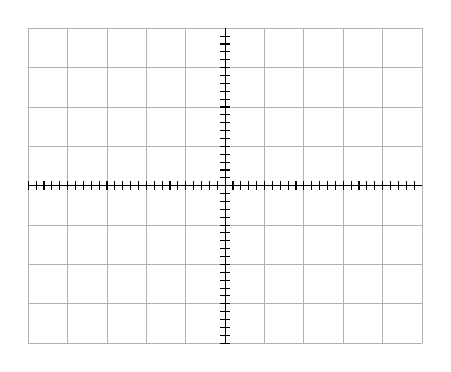
\begin{tikzpicture}
\draw[step=0.5 cm, line width=0.1mm, black!30!white] (0,0) grid (5,4);
\foreach \x in {0,0.1,...,5}{\draw (\x, 1.94) -- (\x, 2.06);}
\foreach \y in {0,0.1,...,4}{\draw (2.44,\y) -- (2.56,\y);}
\draw(0,2)--(5,2);
\draw(2.5,0)--(2.5,4);
\end{tikzpicture}
\end{minipage}

& 
\begin{minipage}{0.5\textwidth}

Sec/div = 

~~

Volts/div = 

~~

Measured Period (horizontal squares times sec/div) = 

~~

Measured Amplitude (vertical squares times volts/div) = 

\end{minipage}
\\
\end{tabular}


\item Show the calculation of the frequency based on the period you measured. Is this close to what you expected? 
\begin{displaymath}
f = \frac{1}{T} = 
\end{displaymath}

\jump{1}

\item What happens to the image on the oscilloscope when you change the frequency on the signal generator? 

\jump{1}

\item What happens when you change the sec/div dial. Describe how this is fundamentally different than above. (Hint: What if you were measuring the frequency of the signal)?

\jump{1}

\pagebreak

\item What happens to the image on the oscilloscope when you change the amplitude of the signal on the signal generator? 

\jump{1}

\item Describe what happens when you change the volts/div dial. How is this different than changing the amplitude on the signal generator?

\jump{1}






\item \textit{Predict} with a calculation, the frequency at which you would set the signal generator so that on a Sec/div of 0.5 ms (recall 1 ms = \SI{1E-3}{s}) so exactly 2 complete waves would fit on a sweep: 

\jump{1}

\item Set the frequency generator to your predicted value. Verify that your prediction was close and sketch the view of the oscilloscope below. (If you were considerably off, see if you made an error above and correct it.) 
\begin{center}
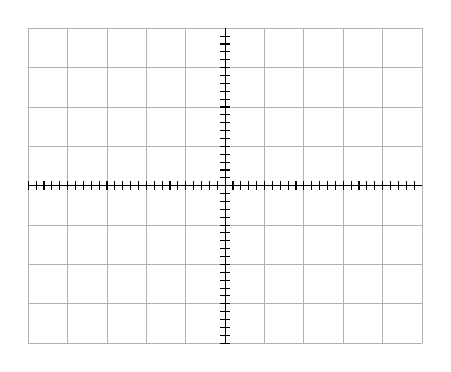
\begin{tikzpicture}
\draw[step=0.5 cm, line width=0.1mm, black!30!white] (0,0) grid (5,4);
\foreach \x in {0,0.1,...,5}{\draw (\x, 1.94) -- (\x, 2.06);}
\foreach \y in {0,0.1,...,4}{\draw (2.44,\y) -- (2.56,\y);}
\draw(0,2)--(5,2);
\draw(2.5,0)--(2.5,4);
\end{tikzpicture}
\end{center}

volts/div = 
~\\
~\\

time/div = 

\pagebreak

\subsection*{IIb.Lissajoui figures}

We can plot one signal along the x-axis and the other signal along the y-axis, by selecting the X-Y feature on the timing. The result is a Lissajous figure. Lissajous figures tells us about the phase difference between the two signals and the ratio of their frequencies. You may find it difficult to maintain the Lissajous figures in a fixed configuration because the two oscillators are not phase and frequency locked. Their frequencies and phase drift slowly causing the two different signals to change slightly with respect to each other. Sketch the output of the following in X-Y mode, note what happens as the phase changes. 

\begin{enumerate}
\item {2 signals with the same frequency (Set both to 100 Hz for example)} How does the shape change as the phase changes? (You can change to the time based mode with the switch at ``E" in the diagram to ``both" to see the signals together and observe their phase.)  
\jump{1}

\item {Signals in  2:1 ratio}
\jump{1}

\item Explore a few more ratios (For example 200 Hz and 300 Hz would be a 2:3 ratio.) Have each group member choose a favorite and list the ratio below:

\jump{1}

\end{enumerate}


 

 











\end{enumerate}



\end{enumerate}
\end{document}



